\chapter{Level2 processor and I/O data}

\begin{figure}[t]
\centering
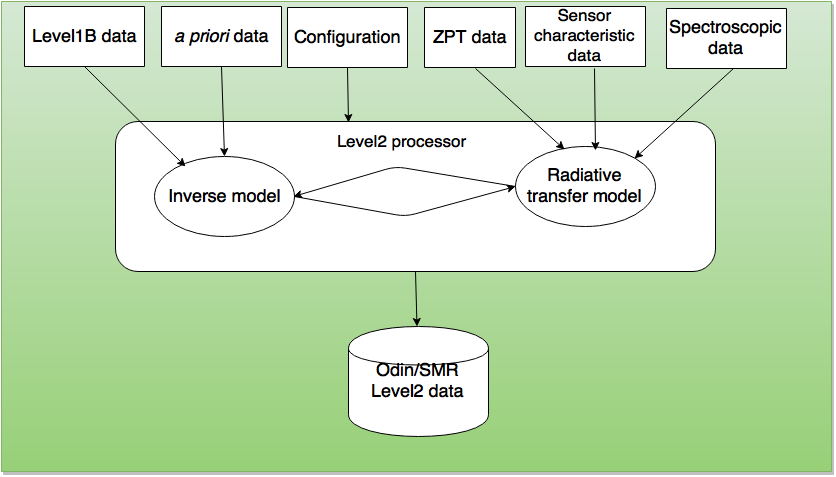
\includegraphics[width=14cm]{smr-level2-processor.png}
\caption{Schematic of the I/O data used and generated by the \smr\ Level2 processor.}
\label{fig:level2}
\end{figure}

\begin{figure}[t]
\centering
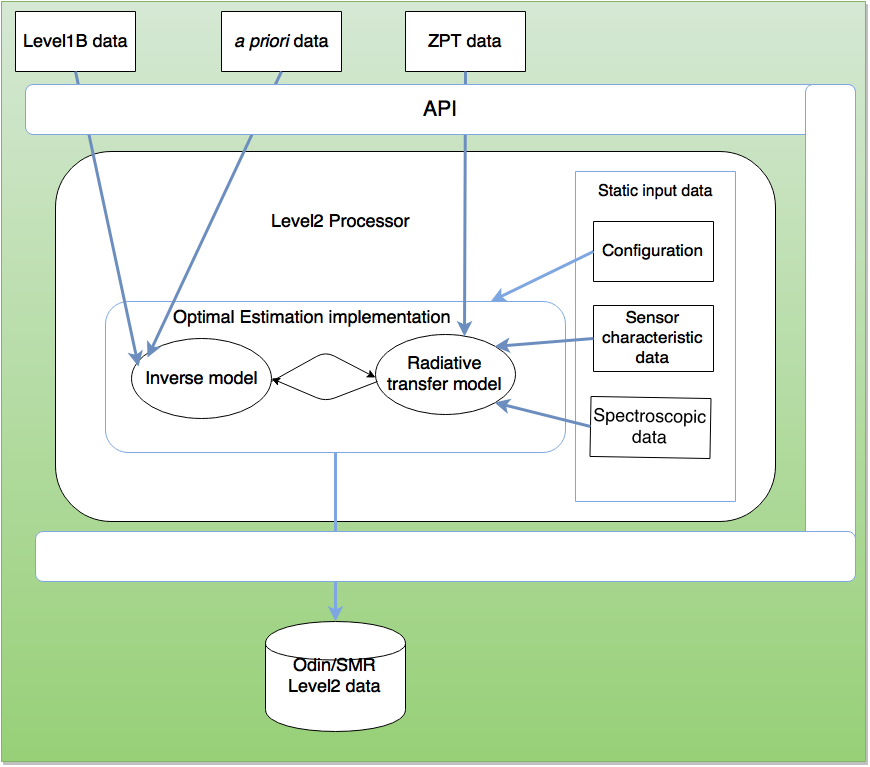
\includegraphics[width=14cm]{smr-level2-processor2.png}
\caption{Schematic of the I/O data used and generated by the \smr\ Level2 processor.}
\label{fig:level2b}
\end{figure}



\section{Level2 processor overview}

The \smr\ Level2 processor is designed to process
measurements from a scan of \smr\ in order to
retrieve profiles of atmospheric species.    
The Level2 processor is an optimal estimation method (OEM)
implementation, which combines measurement
information with Ancillary/Auxiliary data
and applies a forward model, and an iterative
scheme is used to find a best solution.   
The details of the algorithms within the
\smr\ Level2 processor is described in \smr\ Level2 ATBD
\citep{atbdl2}.

\section{Level2 processor input data}

Figure~\ref{fig:level2} describes, on a high level, the input data used
by the Level2 processor and the generated output data.
The input data can be divided into two groups,
dynamic (or semi-dynamic) and static input data,

\begin{itemize}
  \item dynamic (or semi-dynamic) input data:
  \begin{itemize}

    \item \emph{Level1B data}: the most basic input data to the 
    Level2 processor is the Level1B data, i.e. geolocated and 
    calibrated spectra from a scan of \smr.
    
    \item \emph{Climatological \textit{apriori} data}:
    climatology data, covering all species of interest is required, as
    the OEM implementation needs a starting estimate for each profile
    to be retrieved. The climatology covers vertical, seasonal,
    and latitudinal variations of each species and is based on data
    from the "Bourdeaux" climatlogy. %\dots\todo{? Do we have any reference here.}\

    \item \emph{ZPT data}:
    The Level2 processor requires external ZPT data,
    (altitude, pressure, and temperature).
    The ZPT data is extracted from the ERA-Interim dataset for the geolocation
    of the scan. ERA-Interim is a global atmospheric reanalysis from 1979, and
    data is available throughout the Odin mission. The ERA-Interim data used
    has a 0.75\(^\circ\)\ resolution in latitude and longitude and 6\,\(h\)
    in time.
    
    

  \end{itemize}
  \item static input data:
  \begin{itemize}
    \item \emph{Sensor characteristic data}:
    The forward model simulation of the Level2 processor takes into account
    sensor characteristic data, i.e. the antenna angular response,
    sideband filtering, and frequency response of each spectrometer channel.

    \item \emph{Spectroscopic data}:
    Spectroscopic data is basic input to the forward model of the Level2
    processor.

    \item \emph{Configuration}:
    \smr\ applies a number of different observation modes
    (different frequency intervall coverage and scanning altitudes) 
    and for each mode a different configuration is applied
    of the Level2 processor.
  \end{itemize}
\end{itemize}


The Level2 processor obtains the dynamic 
and semi-dynamic input data through a hierarcical
REST API, and the API is described in Sect.~\ref{sec:api}.
The static input data is integrated into the
Level2 processor, as described in Figure~\ref{fig:level2b}. 
%\smr\ applies a number of different observation modes,
%but the Level2 processor is identical for the various modes,
%in terms of the high level workflow.
The detailed data formats of the dynamic 
and static data are described in 
Sect.~\ref{sec:api} and Sect.~\ref{sec:static}.


\clearpage
\newpage
\subsection{API and dynamic input data}
\label{sec:api}

The Level2 processor obtains dynamic input data through
a hierarcical REST API, where deeper URIs return more
specific data. All GET calls return JSON objects.
The call URIs hierachy is organized in the following way:
\begin{itemize}
    \item \url{rest_api/<version>/freqmode/<date>/}: Returns object, which describes which frequency modes that were deployed the
    given date
    \begin{itemize}
        \url{rest_api/<version>freqmode/<date>/<backend>/<freqmode>/}: Returns object, which describes log data of the scans
        for the given date and deployed frequency mode
        \begin{itemize}
           \item \url{rest_api/<version>/scan/<backend>/<freqmode>/<scanID>/}: Returns object that describes Level1B data for a given scan       
           \item \url{rest_api/<version>/ptz/<date>/<backend>/<freqmode>/<scanID>/}: Returns object that describes ptz data for a given scan
           \item \url{rest_api/<version>apriori/<species>/<date>/<backend>/<freqmode>/<scanID>/}: Returns object that describes \textit{a priori} data for a given scan
        \end{itemize}  
    \end{itemize}
\end{itemize}
  
The data returned by the five various GET calls listed above 
is described in the following sections.
Key/value pairs are listed as name of the key
along with the type of the corresponding value within parantheses, followed
by a brief description of the contents.

\subsubsection{Level1B overview data}
\subsection*{\url{rest_api/<version>/freqmode/<date>/}}
Method: \emph{GET}

Returns object, which describes which frequency modes that were deployed the
given date (YYYY-MM-DD), with the following attributes:
\begin{itemize}
    \item Info:

        A list of objects containing information about which
        frequency modes that were mesured this date. 
        Each object contains the following keys:

        \begin{itemize}
            \item Backend \emph{(String)}: The backend for the data
            \item FreqMode \emph{(Int)}: The frequency mode for the data
            \item NumScan \emph{(Int)}: The number of available scans
            \item URL \emph{(URI)}: A URI 
                for getting more specific of the available scans\\ 
                 (\url{freqmode/<date>/<backend>/<freqmode>/})
        \end{itemize}
\end{itemize}

\subsection*{\url{rest_api/<version>/freqmode/<date>/<backend>/<freqmode>/}}
Method: \emph{GET}

Returns object, which describes log data of the scans  
for the given date, backend, and freqmode,
with the following attributes:

\begin{itemize}
    \item Info:

        A list of objects that describes each scan
        with some log data.  
        Each object contains the following keys:

        \begin{itemize}
            \item AltEnd \emph{(float)}: Tangent point altitude ([\,m\,]) for last spectrum in scan
            \item AltStart \emph{(float)}: Tangent point altitude for first spectrum in scan
            \item DateTime \emph{(str)}: Mean UTC datetime (datetime(first) + datetime(last))/2 of scan
            \item FreqMode \emph{(Int)}: Deployed frequency mode
            \item LatEnd \emph{(float)}: Latitude of tangent point for last spectrum in scan
            \item LatStart \emph{(float)}: Latitude at tangent point for first spectrum in scan
            \item LonEnd \emph{(float)}: Longitude of tangent point for last spectrum in scan
            \item LonStart \emph{(float)}: Longitude at tangent point for first spectrum in scan
            \item MJDEnd \emph{(float)}: Modified julian date for last spectrum in scan
            \item MJDStart \emph{(float)}: Modified julian date for first spectrum in scan
            \item NumSpec \emph{(int)}: Number of atmospheric spectra in scan
            \item ScanID \emph{(int)}: Satellite time word identifier of scan
            \item SunZD \emph{(float)}: Mean solar zenith angle  (SunZD(first) + SunZD(last))/2 for scan
            \item URLS a list of key/value describing URIs containing
            more detailed data
            \begin{itemize} 
                \item URL-apriori-<species> \emph{(URI)}: 
                A URI for getting \textit{a priori} data of the scan\\
                (\url{apriori/<species>/<date>/<backend>/<freqmode>/<scanID>/})
                \item URL-ptz \emph{(URI)}: A URI for getting ptz data for the scan\\
                (\url{ptz/<date>/<backend>/<freqmode>/<scanID>/})
                \item URL-spectra \emph{(URI)}: A URI for getting Level1B spectra of the scan\\         
                (\url{rest_api/<version>/scan/<backend>/<freqmode>/<scanID>/})        
            \end{itemize}
       \end{itemize}   
\end{itemize}

\subsubsection{Level1B data}
\subsection*{\url{rest_api/<version>/scan/<backend>/<freqmode>/<scanID>/}}
Method: \emph{GET}

Returns an object that describes the Level1B data of the scan,
with the following attributes (See \citet{atbdl1b} for more details):

\begin{itemize}

  \item Version \emph{(Array of integers)}: Calibration version
  \item Quality \emph{(Array of integers)}: Quality indicator of scan/spectrum
  \item STW \emph{(Array of integers)}: Satellite time word
  \item MJD \emph{(Array of doubles)}: Modified julian date of observation
  \item Orbit \emph{(Array of doubles)}: Orbit number, including fractional part
  \item Spectrum \emph{(2-D Array of doubles)}: Frequency sorted and intensity calibrated spectra
                       in Rayleigh Jeans temperature in Kelvin
  \item TrecSpectrum \emph{(Array of doubles)}: Frequency sorted receiver noise temperature spectrum
                       determined and used in calibration of this scan
  \item Frontend \emph{(Array of integers)}: The frontend used for this observation: 1\,=\,555, 2\,=\,495, 
                       3\,=\,572, 4\,=\,549, and 5\,=\,119
  \item Backend \emph{(Array of integers)}: The backend used for this observation: 1\,=\,AC1 and 2\,=\,AC2
  \item RA2000 \emph{(Array of doubles)}: The right ascension (J2000) of the direction of pointing in degrees
  \item Dec2000 \emph{(Array of doubles)}: The declination (J2000) of the direction of pointing in degrees
  \item Longitude \emph{(Array of doubles)}: Geodetic longitude of the tangent point
  \item Latitude \emph{(Array of doubles)}: Geodetic latitude of the tangent point
  \item Altitude \emph{(Array of doubles)}: Tangent point altitude [m]
  \item GPSpos \emph{(2-D Array of doubles)}: The geocentric position $X$,$Y$,$Z$ in meter of the satellite
  \item GPSvel \emph{(2-D Array of doubles)}: The geocentric velocity $\dot X$, $\dot Y$, $\dot Z$ in meter per 
                         second of the satellite
  \item SunPos \emph{(2-D Array of doubles)}: The geocentric position of the Sun in meter
  \item MoonPos \emph{(2-D Array of doubles)}: The geocentric position of the Moon in meter
  \item SunZD \emph{(Array of doubles)}: The solar zenith angle in degrees
  \item Vgeo \emph{(Array of doubles)}: The velocity of the satellite with respect to the Earth in meter per second
  \item Tcal \emph{(Array of doubles)}: The temperature in Kelvin of the calibration load
  \item Trec \emph{(Array of doubles)}: The mean value of the receiver nosie temperature 
                       in Kelvin used during the intensity calibration
  \item SBpath \emph{(Array of doubles)}: The path length in meter of the SSB diplexer
  \item AttitudeVersion \emph{(Array of integers)}: The version number of the attitude reconstruction software (SODA) 
                         used at SSC during production of attitiude files
  \item FreqRes \emph{(Array of doubles)}: The spacing in Hz between neighbouring channels for this spectrum
  \item FreqCal \emph{(2-D Array of doubles)}:  These are the four local oscillator frequencies of the SSB modules
  \item IntTime \emph{(Array of doubles)}: The integration time in seconds, i.e. the duration of this observation
  \item EffTime \emph{(Array of doubles)}: The effective integration time in seconds, i.e. you will get the
                         noise level in this spectrum by using this time and the receiver noise 
                         temperature from above and the usual radiometer formula:
                        \begin{verbatim}dT = Trec/sqrt(df * EffTime)\end{verbatim}
                         where {\tt df} is the bandwidth (FreqRes) of the spectrometer
  \item Channels \emph{(Array of integers)}: The number of channels in this spectrum
  \item FreqMode \emph{(Array of integers)}: Frequency mode applied
  \item TSpill \emph{(Array of doubles)}: Estimated Tspill in Kelvin
  \item ScanID \emph{(Array of integers)}: satellite time word scan identifier
  \item Apodization \emph{(Array of integers)}: Filter used when converting
    auto-correlations to power spectrum. 1\,=\,no filter, 1\,=\,Hanning 
  \item Frequency \emph{(Object)}: an object that contains information that can be used to create frequency grids for the spectra
                       and consists of following keys: 
  \begin{itemize}             
      \item LOFreq \emph{(Array of doubles)}: Local oscillator frequency in Hz in the rest frame of the
                       observed object, i.e Doppler corrected
      \item AppliedDopplerCorr \emph{(Array of doubles)} The applied Doppler correction in Hz
      \item IFreqGrid \emph{(Array of doubles)}: The frequency grid can be obtained by
                       \begin{verbatim}frequency = LOFreq + IFreqGrid\end{verbatim}
      \item SubBandIndex \emph{(2-D Array of integers)}: The SubBandIndex 
                       can be used to identify from which sub-band a given channel belongs to.
                       An example SubBandIndex array is [[ -1, -1, 420, 509, 111, 1, 310, 200],
                       [-1, -1, 508, 618, 199, 110, 419, 309]].
                       The first and second row indicate the start and end positions, respectively,
                       of the eight sub-bands in the frequency sorted spectrum.
                       The first and second index in these rows corresponds to SubBand 1 and 2, and so
                       on. E.g sub-band 3 data can be found between index 420 to 508.
                       -1 indicates that data from this band is not used.
     \item ChannelsID \emph{(Array of integers)}: Channel identifier describes the location
                       of the sorted channels in the original unsorted spectra
  \end{itemize} 
  \item ZeroLagVar \emph{(2-D Array of doubles)}: Zerolag variation (\([\%]\)) of the surrounding reference measurements for all sub-bands.
                       \begin{verbatim}ZeroLagVar =
abs(diff(ZeroLag))/mean(ZeroLag)\end{verbatim} 
                        ZeroLag is the measured coefficient of the first channel of the auto-correlator,
                        and is proportional to the total power of the band
\end{itemize}



\subsubsection{PTZ data}
\subsection*{\url{rest_api/<version>/ptz/<date>/<backend>/<freqmode>/<scanID>/}}
Method: \emph{GET}

Returns an object that describes the ptz data of the scan,
with the following attributes:

\begin{itemize}
    \item Pressure \emph{(array of doubles)}: Pressure vector ([\,Pa\,])
    \item Temperature \emph{(array of doubles)}: Temperature vector([\,K\,])
    \item Altitude \emph{(array of doubles)}:  Altitude vector([\,m\,])
    \item Latitude \emph{(double)}: Latitude of PTZ data
    \item Longitude \emph{(double)}: Longitude of PTZ data
    \item MJD \emph{(double)}: Modified Julian Date of PTZ data

\end{itemize}

\subsubsection{Climatological \textit{apriori} data}
\subsection*{\url{rest_api/<version>/apriori/<species>/<date>/<backend>/<freqmode>/<scanID>/}}
Method: \emph{GET}

Returns an object that describes the \textit{a priori} data of the scan,
with the following attributes:

\begin{itemize}
    \item Pressure \emph{(array of doubles)}: Pressure vector ([\,Pa\,])
    \item VMR \emph{(array of doubles)}: Climatology volume mixing ratio vector [\,--\,] of the species
    \item Species \emph{(String)}: description of species, i.e. one of 'BrO', 'Cl2O2', 'CO',
          'HCl', 'HO2', 'NO2', 'OCS', 'C2H2', 'ClO', 'H2CO', 'HCN', 'HOBr', 'NO', 'OH', 'C2H6',
          'ClONO2', 'H2O2', 'HCOOH', 'HOCl', 'O2', 'SF6', 'CH3Cl', 'ClOOCl', 'H2O', 'HF', 'N2', 'O3',
          'SO2','CH3CN', 'CO2', 'H2S', 'HI', 'N2O', 'OBrO', 'CH4', 'COF2', 'HBr', 'HNO3', 'NH3', or 'OClO'.
\end{itemize}



\subsection{Static input data}
\label{sec:static}
Static data (sensor characteristic data, spectroscopic data, and configuration)
is required by the Level2 processor, although this data is in a strict
sense not input data to the Level2 processor, as this data
is contained by the Level2 processor as explained by Figure~\ref{fig:level2b}.
The sensor characteristic and spectroscopic data
is used by the forward model (ARTS) of the Level2 processor,
and the configuration controls the complete retrieval
calculation including the forward model calculation.  
The static data used by the Level2 processor is 
described in the following sections.
 

\subsubsection{Configuration}

The \smr\ retrievals are performed by a Matlab implementation of OEM,
that is a part of the Atmlab package (available at \url{www.radiativetransfer.org/tools}).
The main OEM function in Atmlab is \emph{oem.m}. 
The Atmlab package contains the required functions to interface \emph{oem.m} with ARTS
(i.e. read/write ARTS output/input files).
The OEM implementation is controlled by a Matlab object
(a Matlab structure denoted as Q), and  
a description of this structure is found in Appendix~\ref{sec:dataformat}.
Part of this setting is general for all of the various 
observation modes applied by \smr\, while some of the settings
are observation mode specific.

\subsubsection{Sensor characteristic data}

\subsubsection*{Antenna angular response}
%\begin{table}
%\caption{ Frequency mode and antenna angular response function file relationships.}
%\label{table:antenna}
%\begin{tabular}{|l|l|l|}
%\hline
%\textbf{Frequency} & \textbf{Integration} & \textbf{Antenna Response function file} \\
%\textbf{mode} & \textbf{time [ms]} &  \\
%\hline
%  01 & 860  & qsmr/DataFiles/Antenna/antenna\_fmode01\_tint0860ms.xml \\ \hline                                                                      
%  01 & 1860 & qsmr/DataFiles/Antenna/antenna\_fmode01\_tint1860ms.xml \\ \hline                                                               
%  01 & 3860 & qsmr/DataFiles/Antenna/antenna\_fmode01\_tint3860ms.xml \\ \hline                                                                
%  02 & 860  & qsmr/DataFiles/Antenna/antenna\_fmode02\_tint0860ms.xml \\ \hline                                        
%  02 & 1860 & qsmr/DataFiles/Antenna/antenna\_fmode02\_tint1860ms.xml \\ \hline                                
%  02 & 3860 & qsmr/DataFiles/Antenna/antenna\_fmode02\_tint3860ms.xml \\ \hline                                
%  21 & 860  & qsmr/DataFiles/Antenna/antenna\_fmode21\_tint0860ms.xml \\ \hline       
%  21 & 1860 & qsmr/DataFiles/Antenna/antenna\_fmode21\_tint1860ms.xml \\ \hline
%  21 & 3860 & qsmr/DataFiles/Antenna/antenna\_fmode21\_tint3860ms.xml \\ \hline
%\end{tabular}
%\end{table}

A number of data files describing the antenna pattern
are contained by the Level2 processor.
A given file is valid for a specific frequency mode and integration
time, and the file naming convention is:\\
\url{qsmr/DataFiles/Antenna/antenna_fmode<XX>_tint<YYYY>ms.xml}\\
where \emph{XX} describes the frequency mode (e.g 01, 02, and so on)
and \emph{YYYY} describes the integration time (e.g 0860, 1860, or 3860).
These files are valid for an "azimuthally collapsed"
antenna. The file format is ARTS xml GriddedField4 (see ARTS user guide ~\citep{artsug}),
where the grids are \emph{Polarisation}, \emph{Frequency}, \emph{Zenith angle},
and \emph{Azimuth angle}, and the only non-scalar grid is \emph{Zenith angle}.
An example is given below:

%The ~\citet{artsug}
%Table~\ref{table:antenna} displays antenna response function files,
%contained by the Level2 processor,
%that are valid for different frequency modes and integration 
%times. These files are valid for an "azimuthally collapsed" 
%antenna. The files are stored in ARTS xml format, which is
%described below:
%
\lstset{language=XML}
\begin{lstlisting}
<?xml version="1.0"?>
<arts format="ascii" version="1">
  <GriddedField4 name="Antenna response function">
    <Array name="Polarisation" type="String" nelem="1">
      <String>
          "1"
      </String>
    </Array>
    <Vector name="Frequency" nelem="1">
      5.4482500e+11
    </Vector>
    <Vector name="Zenith angle" nelem="161">
      -2.0000000e-01
      -1.9750000e-01
      ...
      2.0000000e-01
    </Vector>
    <Vector name="Azimuth angle" nelem="1">     
       0.0000000e+00
    </Vector>
    <Tensor4 name="Response" nbooks="1" npages="1" nrows="161" ncols="1">
      3.2714490e-04
      3.4765317e-04 
      ...
      3.4187888e-04 
    </Tensor4>
  </GriddedField4>
</arts>
\end{lstlisting}

\subsubsection*{Sideband filtering}


\smr\ operates as a single sideband receiver. The nominal sideband suppression
is better than 19 dB across the image band, but the actual in-flight sideband
leakage is not perfectly known. The sideband leakage has been estimated to vary
between the frequency modes. The sideband leakage assumed in the retrieval
caclulation is controlled by the configuration parameter
\emph{SIDEBAND\_LEAKAGE}, which describes the relative contribution of the
sideband. So far the sideband leakage is assumed to be flat over each frequency
band.

\subsubsection*{Frequency response of each spectrometer channel}

The frequency response function of each spectrometer channel is contained by
the file \url{qsmr/DataFiles/Backend/backend\_df1000kHz\_withHan.xml} of the
Level2 processor. The response function by itself is determined from the
algorithm that is applied to calibrate \smr\ spectra, i.e. if a Hanning
smoothing is applied or not. The file format is ARTS xml GriddedField1 (see
ARTS user guide ~\citep{artsug}), where the grid is \emph{Frequency}, and an
example is given below:

\lstset{language=XML}
\begin{lstlisting}
<?xml version="1.0"?>
<arts format="ascii" version="1">
  <Array type="GriddedField1" nelem="1">
    <GriddedField1 name="Backend channel response function">
      <Vector name="Frequency" nelem="45">
        -4.8125000e+06
        -4.5937500e+06
        ...
        4.8125000e+06
      </Vector>
      <Vector name="Response" nelem="45">
        -1.6581976e-03
        -3.2984437e-03
        ...
        -1.6581976e-03
      </Vector>
   </GriddedField1>
  </Array>
</arts>
\end{lstlisting}


\subsubsection{Spectroscopic data}

Spectroscopic data is basic input to the forward model (ARTS) applied.
The absorption data used in the calculation is extracted 
from an absorption cross-section look-up table for a computational efficiency reason.
The abosrption look-up table is contained by the Level2 processor.
ARTS provides methods to create, read and write, and 
extract data from the lookup table.
The format of the absorption look-up table and how to create it
is described in details in \citet{artsug}.

%The absorption depends on pressure at a first order, 
%and to a second order of temperature and concentration of absorbing species.
%\subsubsection*{Absorption models}


\section{Level2 processor Output Data}

The output of the OEM implementation of the Level2 processor is
two Matlab objcets (L2 and L2I), where L2 contains
the main results of the retrieval and L2I describes
auxiliary instrument and retrieval data \citep{atbdl2}.
The Level2 processor posts this data to the API
(the \emph{POST} URL is \url{rest_api/<version>/level2})
which in turns store the data in a \smr\ Level2 database.
%The Level2 data can then be obtained from API GET calls
%(in the form of JSON objcets or netCDF files)
%\dots\todo{?.}\
The L2 and L2I objects are described in the following sections.

\subsection{Level2 data}
%\subsection*{\url{rest_api/<version>/level2}}

%The L2 object is "struct array" and contains the following fields (for each retrieved species):
The L2 object is a list of objects (struct array) and each object contains the
keys listed below. Each L2 object describes a single VMR or temperature
profile. For details on how averaging kernel matrix, measurement response and
errors are calculated, see \citep{atbdl2}.

\begin{itemize}

    \item AVK (\emph{2-D array of doubles}): Averaging kernel matrix. For
      gas species the averaging kernels for relative changes is given
      ([\%/\%]). For temperature the unit is [K/K].
    \item Altitude (\emph{array of doubles}): Altitude of retrived values [m]
    \item Apriori (\emph{array of doubles}): \textit{A priori} profile used in
      inversion ([-] or [K])
    \item ErrorNoise (\emph{array of doubles}): Error due to measurement
      thermal noise (square root of the diagonal elements of the corresponding
      error matrix) ([-] or [K])
    \item ErrorTotal (\emph{array of doubles}): Total retrieval error, the
      error due to thermal noise and all interfering smoothing errors (square
      root of the diagonal elements of the corresponding error matrix) ([-]
      or [K])
    \item FreqMode (\emph{int}): \smr\ frequency mode of the observation
    \item InvMode (\emph{string}): Inversion mode
    \item Lat1D (\emph{double}): A scalar representative latitude of the retrieval
    \item Latitude  (\emph{array of doubles}): Approximate latitude of each
      retrieved value
    \item Lon1D (\emph{double}): A scalar representative longitude of the retrieval
    \item Longitude  (\emph{array of doubles}): Approximate longitude of each
      retrieved value
    \item MJD (\emph{double}): Mean modified julian date of the observations
      used in the retrievela
    \item MeasResponse (\emph{array of doubles}): The measurement response, defined
      as the row sum of the averaging kernel matrix [-]
    \item Pressure (\emph{array of doubles}): Pressure grid of the retrieved species [Pa]
    \item Product (\emph{string}): Level2 product name
    \item ScanID (\emph{int}): Satellite time word scan identifier
    \item Temperature (\emph{array of doubles}): Best estimate of temperature
      profile [K] (either retrieved or represents the input zpt data)
    \item VMR (\emph{array of doubles}): Volume mixing ratio or retrieved
      profile [-]. Left empty if the L2 object describes a temperature profile
      retrieval.

\end{itemize}



\subsection{Auxiliary data}
%\subsection*{\url{rest_api/<version>/l2idata/<date>/<l2mode>/<scanID>}}
%\dots\todo{this URL does not exist, but we should add the correct one when it exist}\

The L2I object is a scalar structure (i.e.\ valid for a several L2 objects)
and contains the following keys:

\begin{itemize}
  \item BlineOffset (\emph{2-D array of doubles}): Retrieved ``baseline''
    offsets, that differ for each used spectrum and each autocorrelate sub-module
  \item ChannelsID (\emph{array of doubles}): Channel identifier that describes
    which channels that were used in the retrieval [-]. More exactly it
    describes the location of the sorted channels in the original unsorted
    spectra
  \item FitSpectrum (\emph{2-D array of doubles}): Fitted spectrum [K]
  \item FreqMode (\emph{int}): \smr\ frequency mode of the observation
  \item FreqOffset (\emph{double}): Retrieved frequency offset of the LO frequency [Hz]
  \item InvMode (\emph{string}): Inversion mode
  \item L1bQuality (\emph{int}): Quality of L1b data used
  \item LOFreq (\emph{array of doubles}): LO frequency of each each spectrum of
    the scan [Hz]
  \item MinLmFactor (\emph{double}): The minimum value of the Levenberg -
    Marquardt factor during the OEM iterations [-]
  \item PointOffset (\emph{double}): Retrieved pointing offset in degrees
  \item Residual (\emph{double}): The difference between the spectra matching
    retrieved state and used measurement spectra ([K])
  \item STW (\emph{array of doubles}): Satellite time word of each spectrum
    used in the retrieval
  \item ScanID (\emph{int}): Satellite time word scan identifier
\end{itemize}




